
\documentclass[12pt,twocolumn]{article}
\usepackage[margin=2.2cm]{geometry} % see geometry.pdf on how to lay out the page. There's lots.
\usepackage{graphicx}
\usepackage[export]{adjustbox}
\usepackage{lscape}
\usepackage{afterpage}
\usepackage{hyperref}
\hypersetup{
    colorlinks=true,
    linkcolor=blue,
    filecolor=magenta,      
    urlcolor=cyan,
}

%\geometry{a4paper} % or letter or a5paper or ... etc


\newcommand{\sgcomment}[1]{\textcolor{blue}{SG: #1}}
\newcommand{\lat}[1]{\textcolor{blue}{LAT: #1}}
\newcommand{\todo}[1]{\textcolor{blue}{*#1*}}

% \geometry{landscape} % rotated page geometry

% See the ``Article customise'' template for come common customisations

\title{Legacy Data Confounds Modern Studies}
\author{Luke Anderson-Trocm\'e , Simon Gravel}
%\date{} % delete this line to display the current date

%%% BEGIN DOCUMENT
\begin{document}

\onecolumn
\maketitle
\tableofcontents
\clearpage
\twocolumn
			\section{Introduction}
	\subsection{Larger Sample Sizes}			
The last 5 years has seen an increase in the number of individuals genotyped through private companies or medical research cohorts. 
Larger sample sizes allow researchers to identify finer resolution statistically significant differences between groups of individuals. 
Mutations associated to a disease can be identified by comparing the genomes of healthy individuals to those afflicted by a disease. 
The mutations commonly found in patients and rarely in controls might be associated to the disease in question.
However, demonstrating that these mutations are biologically relevant can be difficult.
Especially with the increasing size of cohorts, spurious associations are increasingly becoming an issue. 
For this reason, careful consideration must be taken when including individuals from different ancestral origins in these association studies.
Benign mutations at high frequencies in one populations might be exceedingly rare in another population.
Therefore, population wide differences in mutations must be included as covariates to avoid spurious associations.

	\subsection{Imputation}
Genome wide associations using large cohorts have lead to developments in the identification of rare genetic diseases as well as the risk prediction to certain types of cancer and diseases. 
Despite drastic reductions in cost of whole genome sequencing, it remains an expensive test for large sample sizes.
For this reason, genotype data is often imputed to increase power for association studies in a cost effective way.


Imputation of genotype data is a probabilistic method that infers the bases of a given genome based on its similarity to a set of reference genomes.
While on average, two humans differ in about 1/10,000 bases, this number is \todo{lower} in closely related individuals, and \todo{higher} in individuals from different continental origins.
Modern chip sequencing will provide the genotype information for over 1 million bases of the genome.
The unique combination of genotyped bases can be enough to identify haplotype blocks that are identical by descent in individuals form the reference database.


The accuracy of imputation depends on the size of the reference database; this varies significantly from one population to another.
This means that individuals with ancestry that is less well represented in the reference database will have lower accuracy of imputation.
To overcome this bias, reference databases are often combined to increase the sample size and in turn, the accuracy of imputation.


Combining data can be an issue when the quality of the data produced can vary between sequencing technologies and even sequencing centres.
The errors in one dataset don't disappear when they are combined with another higher quality one. 
Many of the legacy datasets produced using dated sequencing technologies have been known to contain a higher rate of false positives than their more recent counterparts.
Is it time to retire legacy data? 

	\subsection{Mutation Spectra} 
A genome wide mutational signature can be measured by taking the sum of all the different types of mutations in an individual. 
The signatures from individuals in the same population will have a tendency to be more similar due to shared ancestry.
Harris et al have recently posited that there are patterns of mutations that differ across human populations.
They argued this by showing relative differences in mutational types between and even within continental populations.
In particular, there is \todo{15 percent} more TTC to TCC mutations in people of European descent.
\lat{more here about mutation spectra}

	\subsection{Context}
This project was motivated by an unusual population genetics observation in a recent publication by Harris et. al, that the 1000 Genomes Project (1kGP) Japanese population seem to be partitioned in two clusters of diff mutation rates. 
This heterogeneously distributed mutational signal was unexpected as a signal of this nature could either be due to population structure, a recent mutagen, or technical bias.
In investigating this mutational signature, we were unable to reproduce the results using a larger and higher quality dataset and concluded that this signal can be attributed to sequencing error.


This study is the result of an investigation in the quality of the 1kGP dataset.
To begin, we will discuss the discrepancy between the Japanese samples from the 1kGP and a more recent high quality dataset. 
We then consider methods to discriminate sequencing errors resulting from dated technologies.
Next, we explore more broadly how low quality variants remain embedded in other populations of the 1kGP.
Finally, we will discuss the impact these variants have on modern analyses.


			\section{Results}
	\subsection{A heterogeneously distributed mutational signal}			
Upon comparing the allele frequencies between the two datasets, we observed an unusually large number of private SNPs despite both cohorts being from the same population.
Surprisingly, the SNPs responsible for the signal observed by Harris et. al (2017) were missing in the more recent dataset. 
\todo{plot SFS NAG vs JPT}
We also noticed that the individuals carrying these mutations all had lower average quality scores.
This suggested that individuals with lower quality were driving this signal.
\todo{plot PC1 vs Qual}


To further investigate	 the extent to which low quality individuals were associated to spurious mutations, we performed a genome-wide association (GWA) study  \ref{Figure2}. GWA studies are commonly used to find genomic regions associated to biologically relevant traits. In this case, we are using this analysis in a more unconventional way to identify regions of the genome that are associated to biologically irrelevant traits like SNPs associated to individuals with low quality.
 
Using the linear GWAS function offered by PLINK, we were able to identify \todo{000 $10^{-8}$ and 000 $10^{-6}$} SNPs that were associated to the average quality of SNPs mapped for an individual \ref{Figure2}.  This GWAS included 104 individuals, \todo{000} of them were sequenced in phase 1 while the rest were sequenced in phase 3 of the 1000 Genomes Project.

\todo{does getting rid of these SNPs get rid of the signal? What is the lowest frequency SNP that is statistically significant?}

	\subsection{Average quality of mapped snps Quality Over Time}
As one would expect, the sequencing quality of individuals increases over time \ref{Figure1}. Sequencing centers improve on their laboratory techniques and sequencing technologies improve from one generation to the next. The magnitude and impact of the differences in quality within and between populations has not yet been explored. 

\begin{figure*}
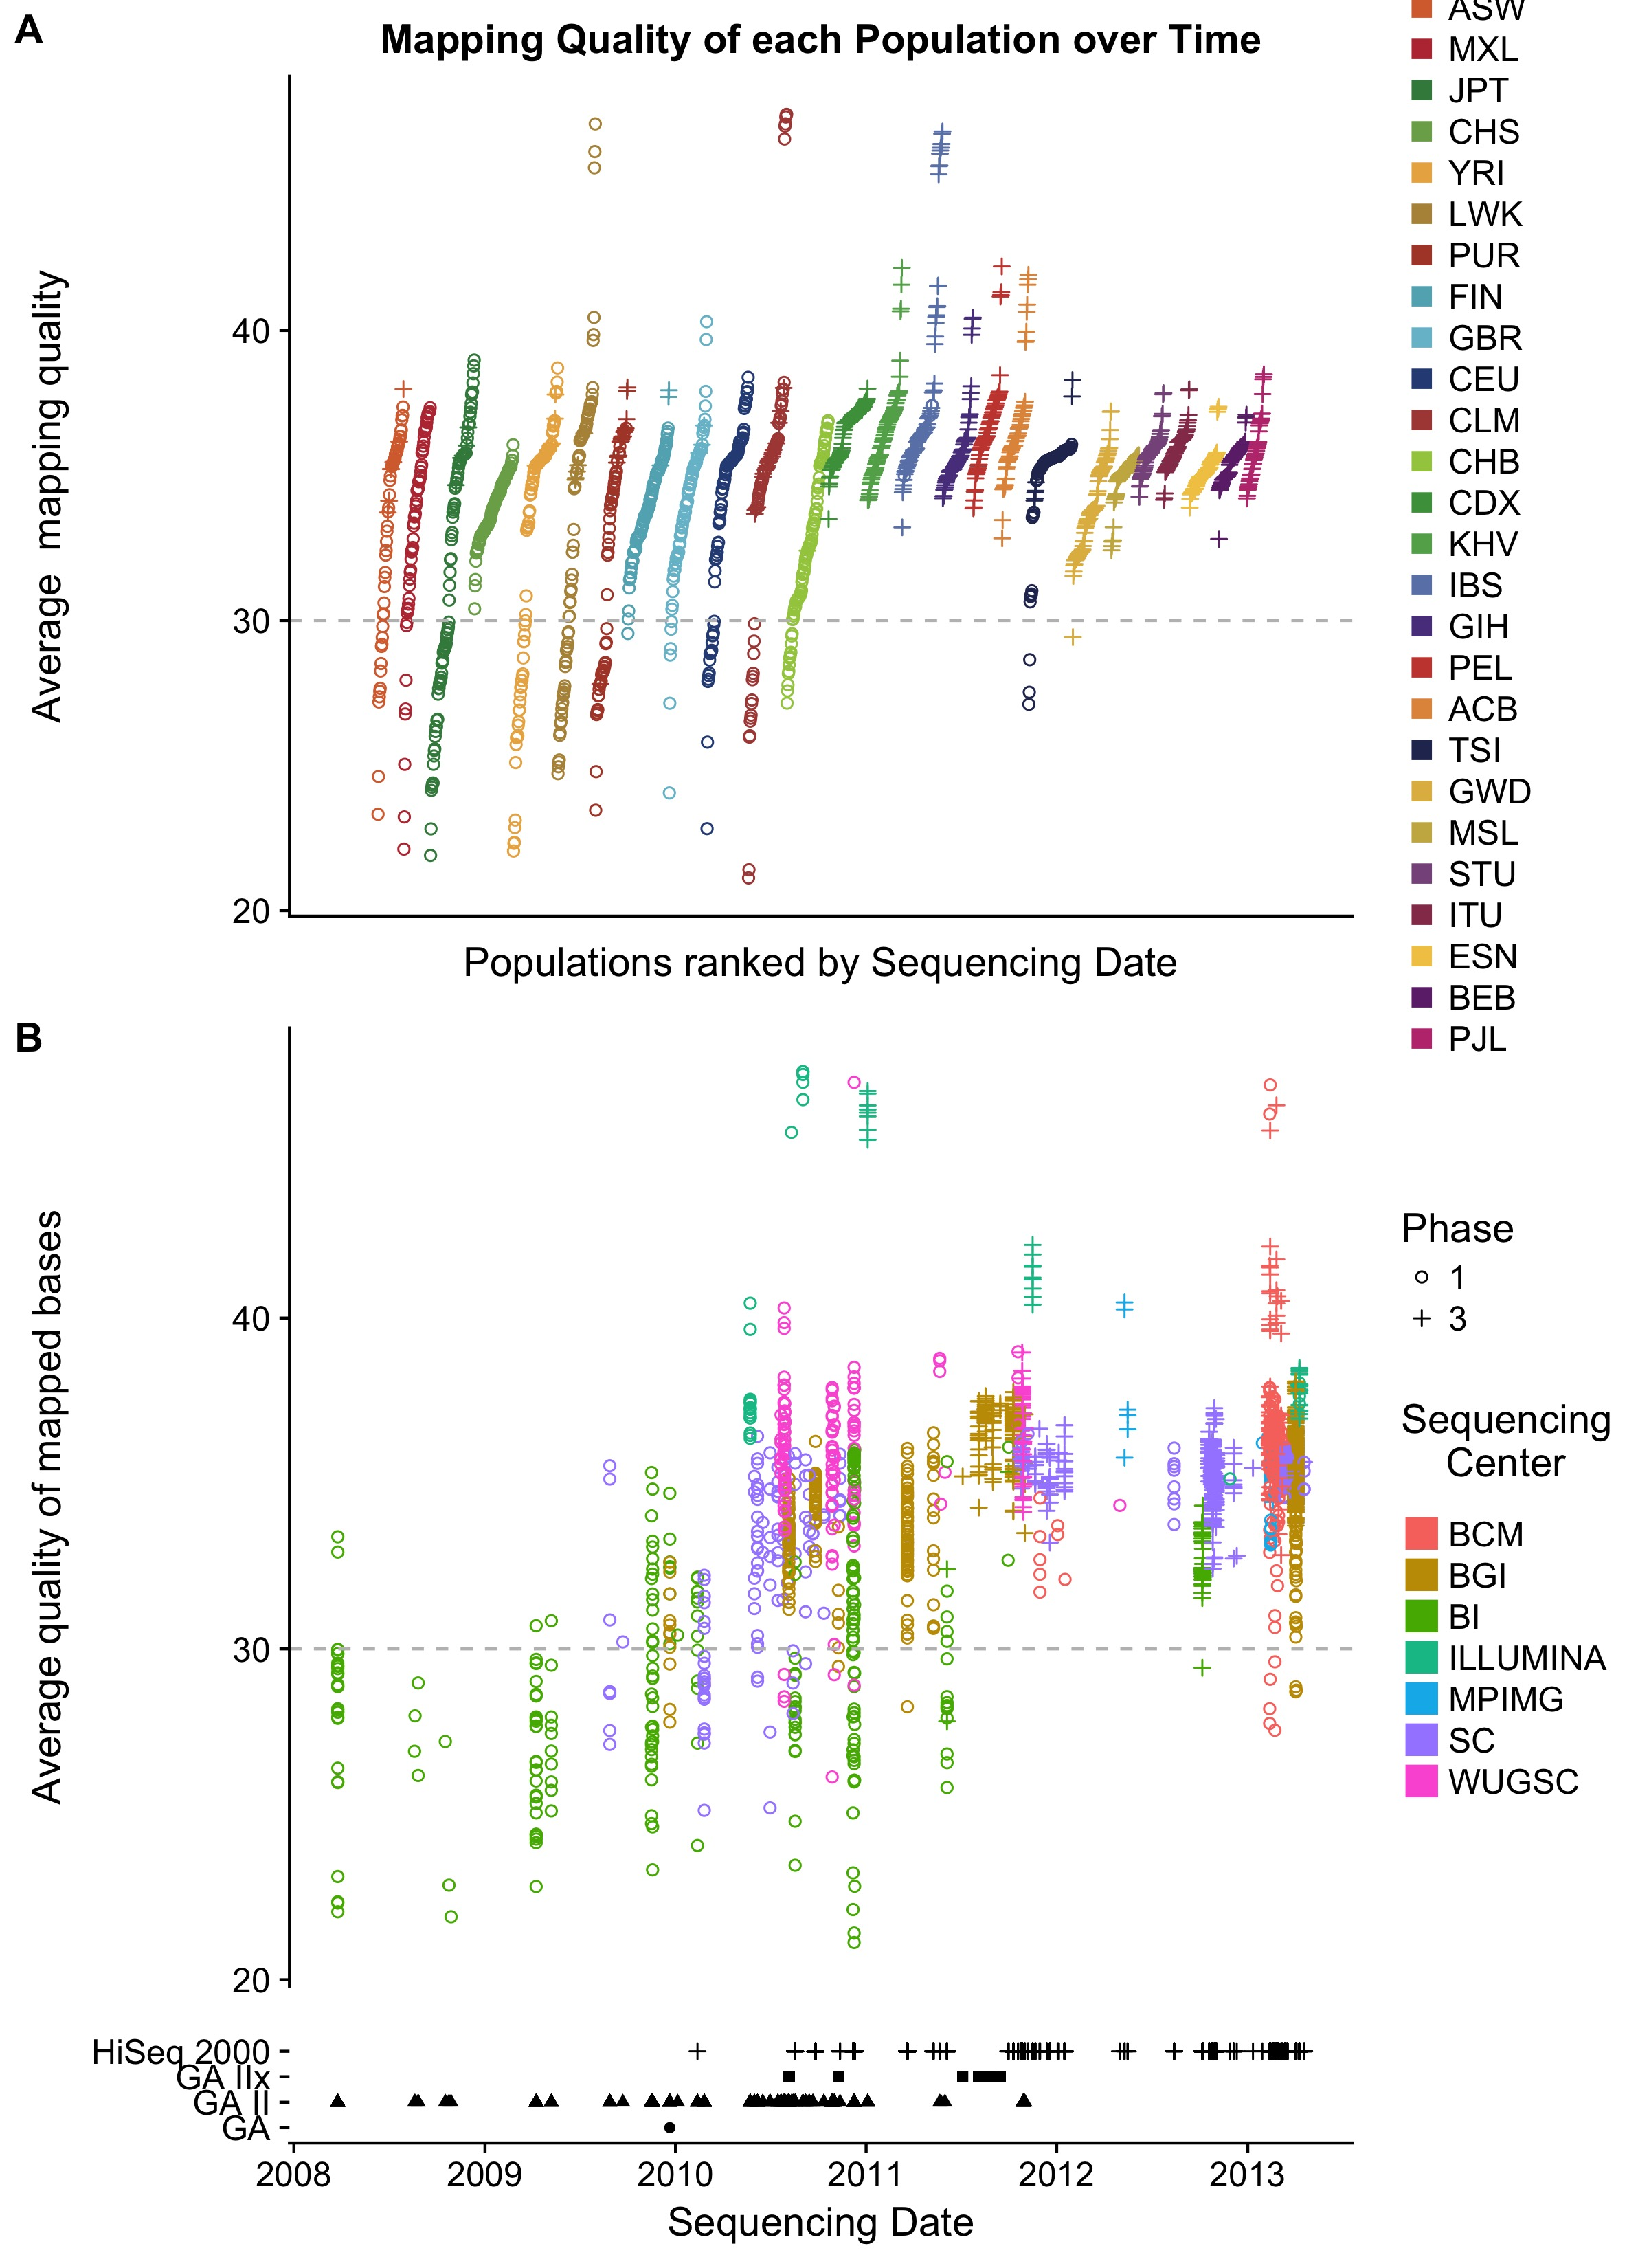
\includegraphics[width=\hsize,keepaspectratio]{MapQualOverTime.jpg}

\caption{A) The average mapping quality of each individual per population included in the 1000 Genomes sequencing project. The average mapping quality per individual was obtained from the raw alignment index data for each sample. The X axis is ranked by populations with the lease to the most variance, followed by average mapping quality per individual. B) Same data as in A) except the X axis is now sorted by sequencing date, and the colors indicate the sequencing centers that produced the data for each individual.}
\label{Figure1}
\end{figure*}

	\subsection{Genome Wide Association}


\begin{figure*}
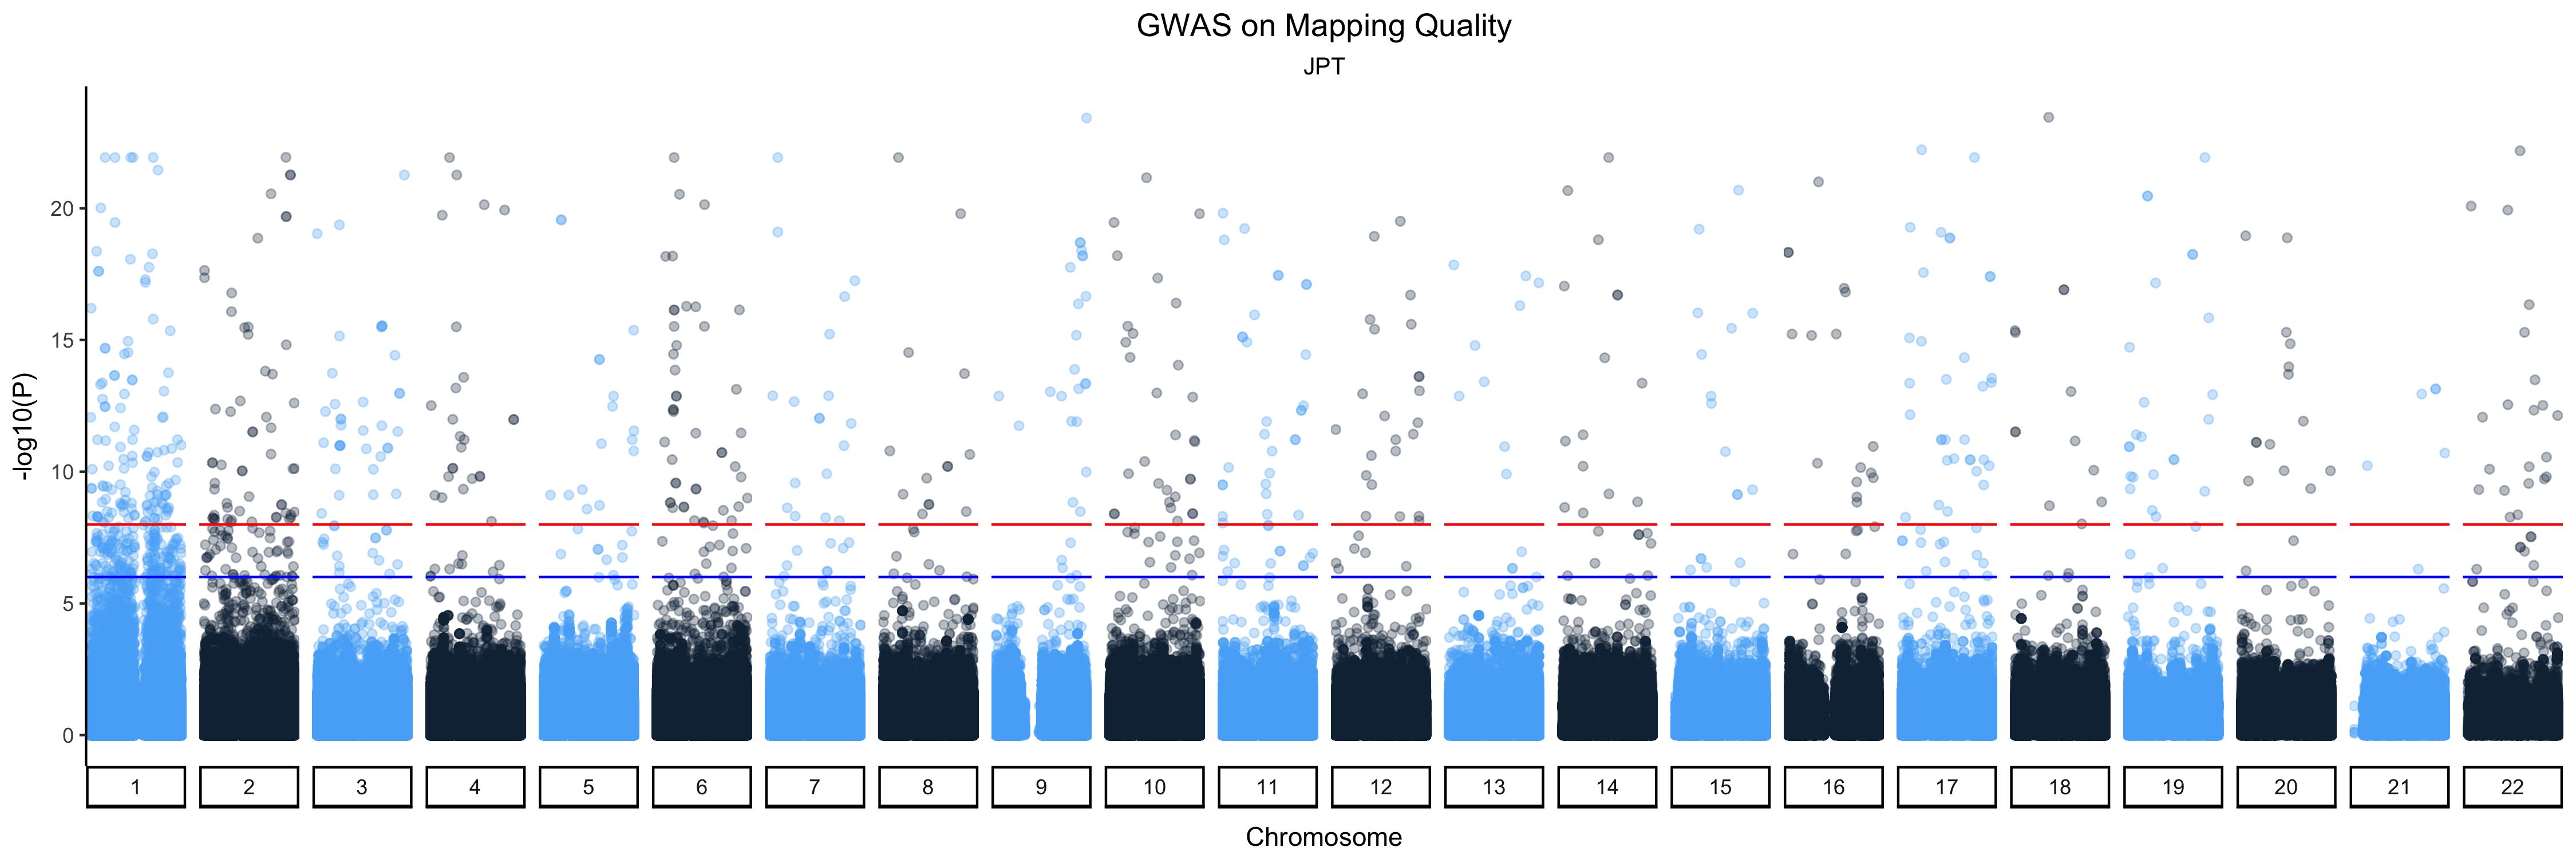
\includegraphics[width=\hsize,keepaspectratio]{GWAS_Qual_GenomeWide_JPT.jpg}
\caption{Genome wide association of the average quality of mapped bases for the Japanese individuals included in the 1000 Genomes Project. This GWAS included 104 individuals, \todo{000} of them were sequenced in phase 1 while the rest were sequenced in phase 3 of the 1000 Genomes Project. The same analysis was performed independently for each of the populations in the 1000 Genomes Project. }
 \label{Figure2}
\end{figure*}

	\subsection{Overlap of Significant SNPs}
Comparing the results of each independent GWAS, we were able to identify over 0000 variants that were independently associated to low quality in multiple populations. This confirmation using more than one GWAS is a very strong result suggesting that these variants might not be legitimate  \ref{Figure3}. 

\begin{figure*}
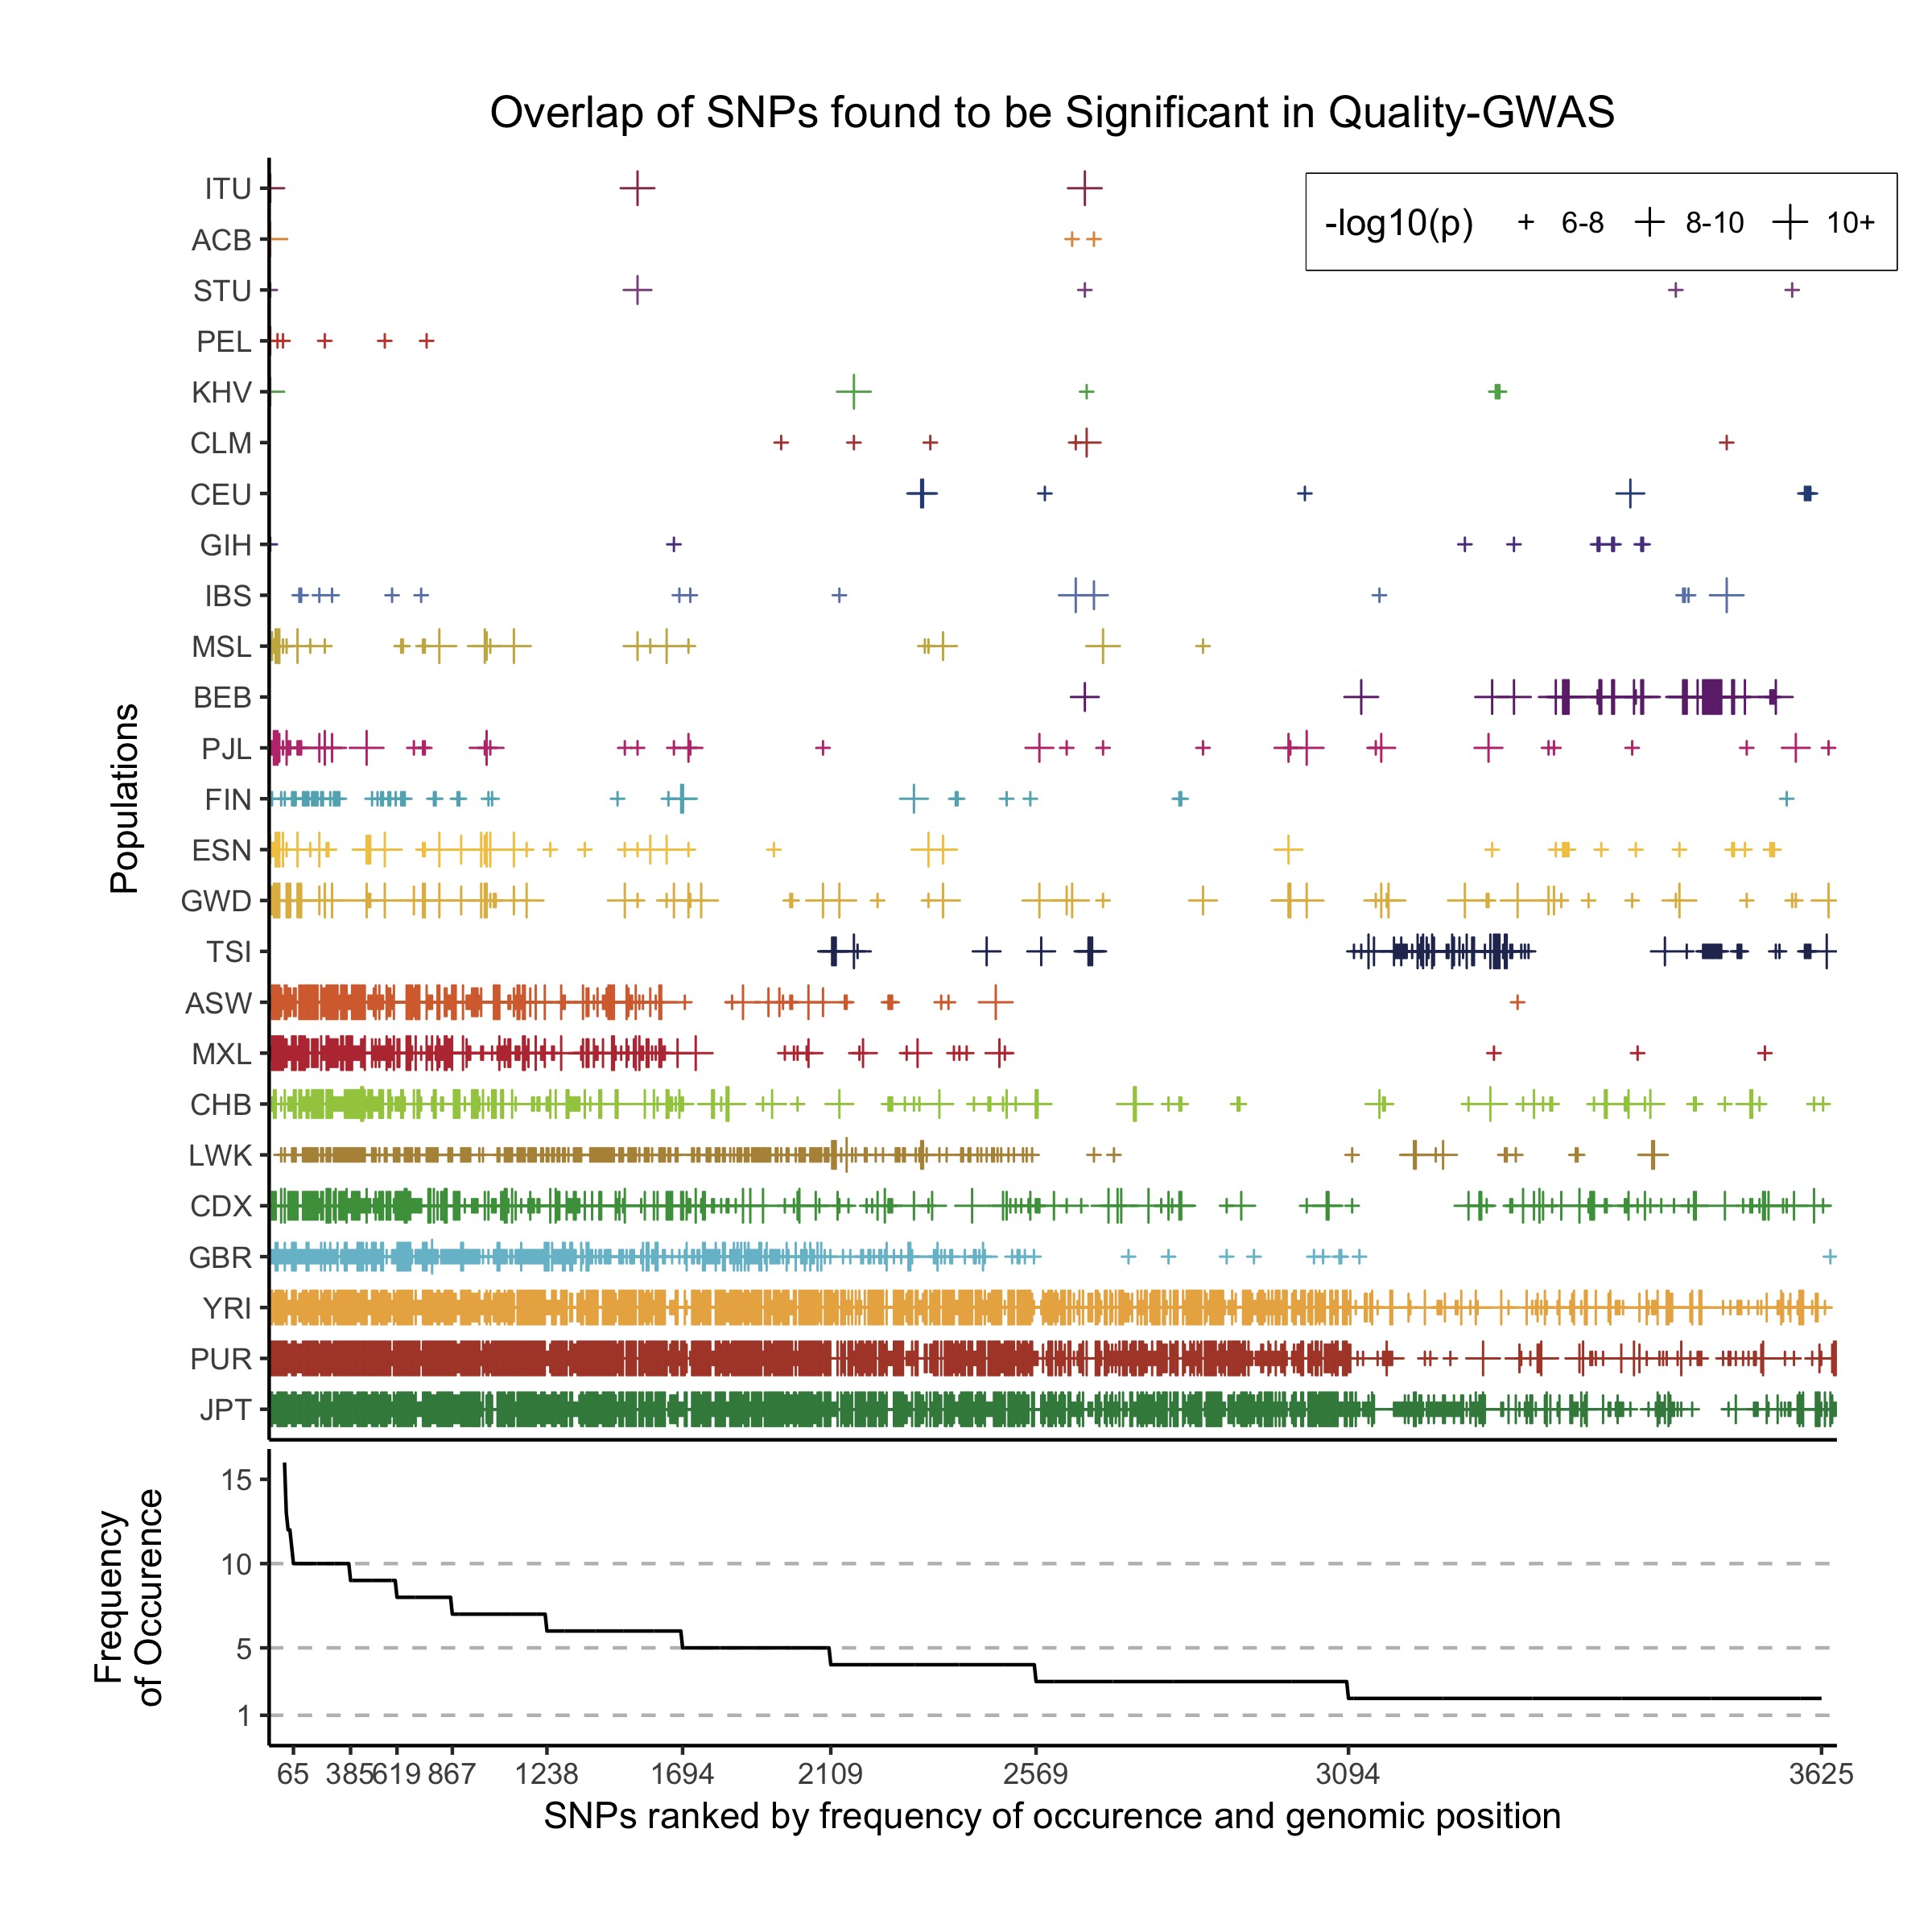
\includegraphics[width=\hsize,keepaspectratio]{SNPOverlap6.jpg}

\caption{Overlap of SNPs identified independently to be associated with quality. Not surprisingly, the populations that have the most low-quality individuals also have the most low-quality variants. What is interesting here, is that the same variants identified as being low quality independently in each population are found in other populations. }
  \label{Figure3}
\end{figure*}

	\subsection{Significant SNPs}
When we remove individuals below a quality of 30, population structure is clarified. 
The signal identified in Harris et. al is enriched in sites associated with low quality
Therefore, when these low quality sites are removed, the mutational signal is also removed. (Or in this case when we remove the individuals with qualities below 30.)

	\subsection{Higher quality datasets don't have these SNPs}

Interestingly, the SNPs we identified had already been removed in higher quality datasets. 
These HQ datasets also have filtered more SNPs than the GWAS was able to identify. 
When we compare the allele frequencies between the 1000 Genomes project Japanese population to a more contemporary dataset, there are many more sites that are enriched with the same mutational signature as described above that are not identified using a GWAS. 
This suggests that we lack the power to identify all the questionable variants from these legacy datasets. 

	\subsection{Imputation}
~30\% of the SNPs we identified as being associated with low quality were found to be imputed using the Michigan Imputation Server. These  should be removed from reference database

	\subsection{Found to be included in other GWAS}
Once we identified SNPs that were clearly associated with low quality, we searched the literature for any GWA studies that might have called these erroneous variants as being significantly correlated with some biological trait. 
Using the NHGRI-EBI Catalog of published genome-wide association studies we queried the rsIDs of the SNPs we identified as being low quality and found 6 recent publications that had found at least one of the variants to have reached genome wide significance in their study. 

Five of these studies used the 1000 Genomes Project as the reference database for imputation and one used the 1000 Genomes Project cell cultures and sequence data. 
They used strict quality thresholds, including population genetic statistical tests such as the Hardy-Weinberg equilibrium test, allele frequency differences using reference populations. 
They also removed rare alleles and alleles with high degrees of missingness. 
Despite using the state of the art quality controls, these erroneous variants managed not only to be imputed onto real genotype data, but they also to reach genome wide significance for the traits they were testing for. 

			\section{Discussion}
\subsection{Why do we care?}
These SNPs matter because they reached genome wide significance for medically relevant traits. 
Could lead to false diagnosis at worst, or spurious correlations at least. 
They were not caught sooner because the batch effect of 1000 genomes had never been properly addressed. 

Our GWAS method was able to identify \todo{000} variants that are likely to be false positives.

We compared the number of SNPs identified in the GWAS to the number of sites that differed between our higher quality Japanese dataset and found that 100?\% of the sites were also missing from the Fumi data. 
Because we are running the GWAS on a per-population base, for rarer mutations, we are lacking the power to identify these significant SNPs.  
However, upon comparing the Japanese 1000 Genomes cohort to a higher quality and larger cohort, we identified \todo{000} more variants that are beyond the expected frequency spectrum deviation for individuals from the same population. 
This suggests that while the GWAS approach can identify some of the low hanging bad apples, there are likely more of these false positives nested inside these legacy cohorts. 
The most conservative approach would be to remove all individuals that don't meet the quality threshold. 
In this case, we used a cut off of an average quality of mapped bases over 30. This threshold has been previously used by \todo{000} studies.

\subsection{GWAS from other papers}
Since these variants are present in more than one population from the 1000 genomes project, they are more likely to be associated to biological traits as they would appear to be like any other variant that is shared among multiple populations. 
The only way to distinguish some of these more covert false positives is to use statistical tests associating the quality metrics of each position relative to each individual. 
\subsection{Why were these SNPs even associated in the first place?}
[due to the temporal nature of the batch effects, and because entire populations were sequenced in one centre on one day, the false positives are more likely to cluster with population structure or case/control?]

			\section{Conclusion}
Our method identifies spurious mutations by correlating mutations with data quality metrics. 
We propose including our quality control methods to identify possible false positives in sequencing data. 
We have focused on the 1000 Genomes Project dataset as its quality metrics were feely available, however the issues of quality control are not limited to this one consortium. 
This study only used one dataset and one quality metric, but using this same approach can be used to identify more false positives in many more datasets. 

As more and more large scale genotyping efforts are being imputed on the same legacy datasets, we must scrutinize the quality of the reference databases to avoid the amplification of false positives. 
These results bring forth many questions regarding the reliability of legacy datasets. 
Moreover, since there are so many broad applications of imputation, it frames the question for reference data turnover. 



\section{Methods}
\subsection{Metadata}
The metadata used in this analysis was compiled from each of the index files from the 1000 Genomes file system. 
Average quality of mapped bases per sample was obtained from the BAS files associated with each alignment file. 
Each BAS file has metadata regarding each sequencing event for each sample. 
If a sample was sequenced more than once, we took the average of the each quality score from each sequencing instance. 
The date of completion of each sequencing occurrence was not available, however we managed to find the submission dates and sequencing centres for each sample in the phase3 analysis sequence index file.  
This file also has multiple entries per sample, however, we were unable to match the individual sequencing runs between the bas files and the index file, which lead us to take the average of the quality scores and only kept the earliest sequencing date per sample. 
The dates of the sequencing are only used to plot Figure. \todo:{Average Quality of mapped bases: How was it calculated?}

\subsection{Data Availability}

Index of BAS files \href{http://ftp.1000genomes.ebi.ac.uk/vol1/ftp/data_collections/1000_genomes_project/1000genomes.low_coverage.GRCh38DH.alignment.index}{available here}.
Phase3 analysis sequence index file  \href{http://ftp.1000genomes.ebi.ac.uk/vol1/ftp/phase3/20130502.phase3.analysis.sequence.index}{available here} 
[link to my compiled metadata file here]

\subsection{Quality Controls}
We reproduced the quality control pipelines used by Harris et. al as they applied the current state of the art quality thresholds to remove questionable sequences especially for the high standards for detecting population level differences. 
Several mask files were applied to remove regions of the genome that might be lower quality, or might have very different mutation rates or basepair complexity compared to the rest of the genome. 
The  1000 Genomes \href{http://ftp.1000genomes.ebi.ac.uk/vol1/ftp/release/20130502/supporting/accessible_genome_masks/20141020.strict_mask.whole_genome.bed}{strict mask} was used to remove low quality regions of the genome , highly conserved regions were removed using the \href{http://hgdownload.cse.ucsc.edu/goldenPath/hg19/database/phastConsElements100way.txt.gz}{phastCons100way} mask file and highly repetitive regions were also removed using the \href{http://hgdownload.cse.ucsc.edu/goldenpath/hg19/database/nestedRepeats.txt.gz}{NestedRepeats} mask file from RepeatMasker. 
Furthermore, only diallelic autosomal SNPs were considered, with missingness below 0.01, MAF less than 0.1, and MAF greater than 0.9.

\subsection{Genome Wide Association}

Using PLINK v1.90b4.4 we ran a linear genome wide association study independently for each population of the 1000 Genomes Project. We used the average quality of mapped bases per individual as the phenotype for the analysis. We also controlled for population structure by including the first 4 principle components of a PCA of each population using genotype data. \todo{NOT DONE YET}

\subsection{Mutation Spectrum}
We calculated the mutation spectrum for each list of significant SNPs for each population \todo{NOT DONE YET}

We also compared the mutation spectrum ratio between populations using a modified version of the methods used in Harris et al. 2017. 

\subsection{Imputation}
Using the Michigan Imputation Server, we imputed the genotype data from 1000 Genomes Project




  



\end{document}





We discovered \todo{000} variants that were associated to low mapping quality in \todo{000} individuals from \todo{000} of the 26 populations included in the 1000 genomes dataset. 
One third of these mutations were included in imputation tests. Population specific mutational signatures were also clarified by removing these spurious mutations.

After compiling all the metadata from each 1000 genomes sequencing run, we noticed a correlation between PC1 of the mutation spectrum signal and the average quality of mapped bases per individual. 

Furthermore, when looking at the days when the individuals were sequenced, we noticed that individuals with this mutational signal were sequenced on the same day in the same sequencing centre.
We then turned our attention to the rest of the 1000 Genomes populations and saw that there were similar batch effects in many of these populations.
			























